\chapter{Литературный обзор}\label{ch:ch1}

Соединение \cbo\ имеет пьезоэлектрическую тетрагональную структуру с пространственной группой симметрии \(I\overline{4}2d\) (\textnumero 122), ионы меди занимают два типа позиций (подрешеток) – 4b и 8d. Как видно из рисунка \cref{fig:unit-cell}, пределах подрешетки 4b существует два типа неэквивалентных позиций, отличающихся ориентацией первой координационной сферы ионов кислорода: для меди в центре ячейки искаженный квадрат из кислородов повернут относительно кристаллографической оси \emph{c} на угол \ang{24} по отношению к осям \emph{a} и \emph{b}, а для меди в правом крае рисунка -- на угол минус \ang{24}. Далее в тексте ионы меди в позициях, эквивалентных позиции центрального иона будут обозначаться A1, а остальные -- A2. Просто проверяю: \cud\, \niIon\, \nif. 

\begin{figure}[ht]
	\centerfloat{
		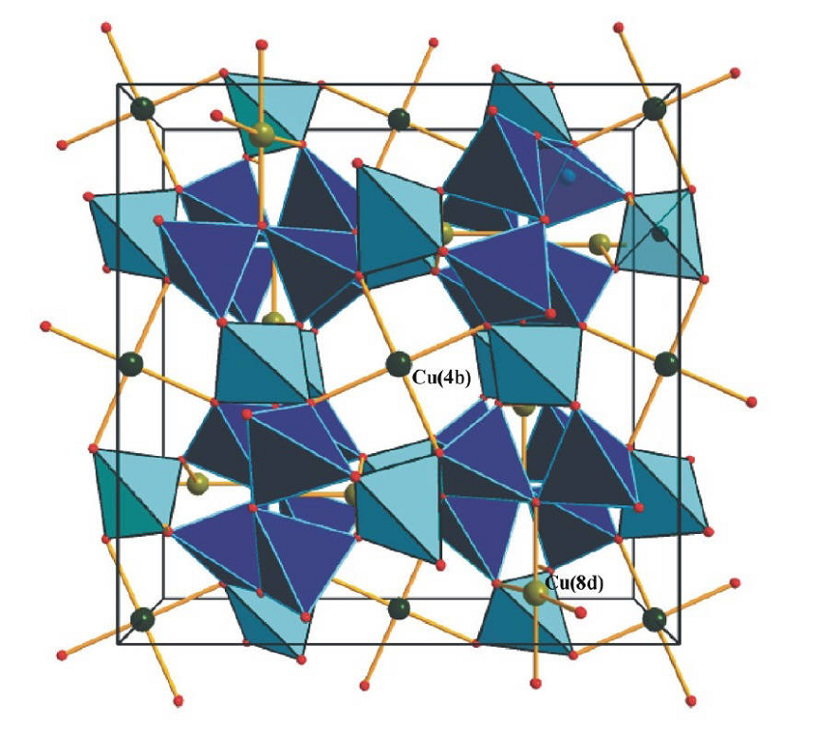
\includegraphics[scale=0.8]{unit-cell}
	}
	\label{fig:unit-cell}
	\caption{Элементарная ячейка \cbo\ \cite{Martinez1971}. Темно- и светло-зелеными кружками изображены ионы \cu\ в позициях 4b и 8d соответственно, красными - ионы O\(^{2-}\), в центрах изображенных тетраэдров находятся ионы B\(^{3+}\). }
\end{figure}

Ионы в подрешетке 8d даже при сверхнизких температурах остаются в парамагнитном состоянии \cite{Boehm2003}, поэтому при описании магнитоэлектрических свойств \cbo\ можно ограничиться рассмотрением лишь позиций 4b. При \SI{9}{\kelvin}<T<\SI{21}{\kelvin} спины ионов в подрешетке 4b  упорядочиваются антиферромагнитно, а при T<\SI{9}{\kelvin} формируется сложная неколлинеарная спиновая структура.  В нулевом магнитном поле спины преимущественно лежат вдоль направления \dir{1}{1}{0}, слегка отклоняясь в направлении \dir{0}{0}{1} \cite{Boehm2003}. Однако при включении уже довольно слабого магнитного поля (\({\sim}500\,\)Э) вдоль направления \dir{1}{1}{0} спины меди в антиферромагнитных подрешетках 4b ориентируется перпендикулярно ему – вдоль направления \dir{1}{\(\overline{1}\)}{0} \cite{Toyoda2019} из-за взаимодействия Дзялошинского-Мория.

\section{Наблюдение статических магнитоэлектрических эффектов}\label{sec:ch1/sec1}

Кристаллическая структура \cbo\ не имеет центра инверсии (точечная группа позиции 4b - \(S_4\)), а при T<\SI{21}{\kelvin} в подрешетке ионов меди 4b нарушается и симметрия по отношению обращению знака времени, поэтому логично заключить, что возможно возникновение магнитоэлектрических эффектов. Однако, попытка обнаружения \emph{статического} магнитоэлектрического эффекта, предпринятая в работе \cite{Nenert2007}, не увенчалась успехом. Авторы наблюдали за изменением диэлектрической проницаемости \cbo\ в широком диапазоне температур (см. рисунок \cref{fig:nenert}), однако никаких характерных изменений диэлектрической проницаемости в точках фазовых переходов не обнаружили -- следовательно, спиновое упорядочение не привело к индуцированию поляризации.

\begin{figure}[ht]
	\centerfloat{
		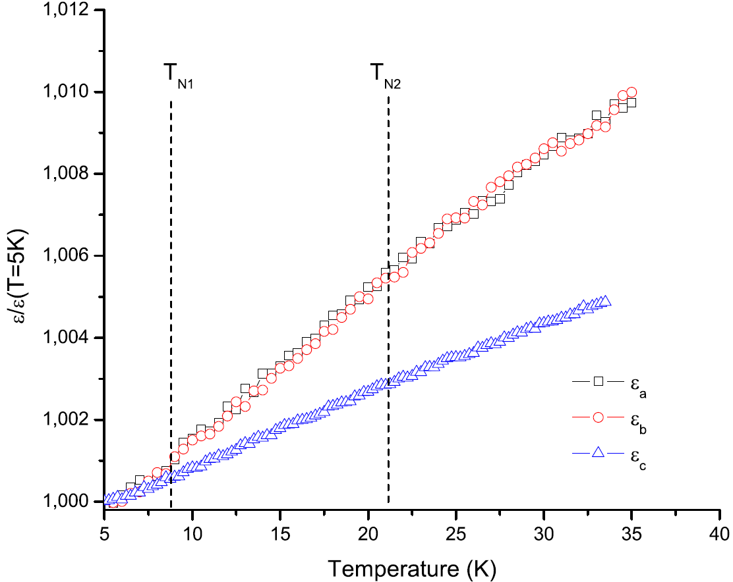
\includegraphics[scale=0.8]{nenert}
	}
	\label{fig:nenert}
	\caption{График зависимости диэлектрической проницаемости \cbo\ от температуры, нормированный на значение $\epsilon$ при \SI{5}{\kelvin} \cite{Nenert2007}.}
\end{figure}

Позднее авторы работы \cite{Khan2013} при изучении бората меди, допированного ионами \niIon\, обнаружили, что в антиферромагнитной фазе при некотором критическом значении внешнего магнитного поля, приложенного в плоскости \textit{ab} кристалла, наблюдается скачок электрической поляризации, причем величина поляризации зависит от направления магнитного поля как \(sin\left(2\theta\right)\), где угол \(\theta\) отсчитывался от направления \dir{1}{0}{0} (см. рисунок \cref{fig:khan}).

\begin{figure}[ht]
	\centerfloat{
		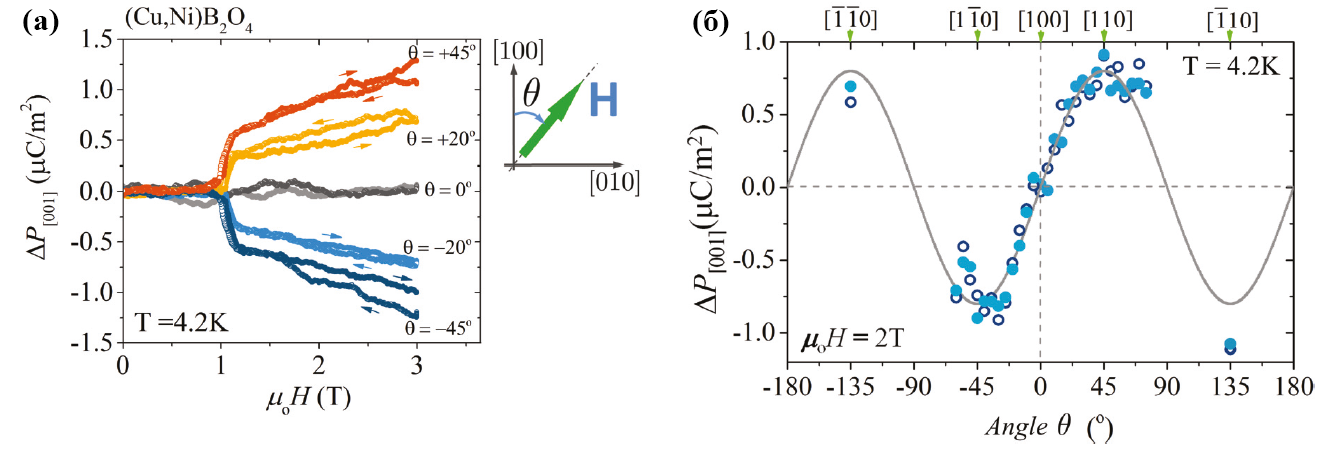
\includegraphics[scale=0.5]{khan2}
	}
	\label{fig:khan}
	\caption{(a) Зависимость величины индуцированной вдоль \dir{0}{0}{1} электрической поляризации в \ncbo\ от величины приложенного магнитного поля для различных его направлений при T=\SI{4.2}{\kelvin} \cite{Nenert2007}. (b) Кружками - экспериментальная зависимость величины электрической поляризации от направления приложенного магнитного поля \SI{2}{\tesla} при T=\SI{4.2}{\kelvin}; сплошная линия - аппроксимация экспериментальных данных графиком функции $A\sin\theta$ \cite{Nenert2007}.}
\end{figure} 

Существующие механизмы магнитоэлектрической связи либо не подходили для описания \cbo\ (обратное взаимодействие Дзялошинского-Мория \cite{Sergienko2006}), либо давали существенно меньшую оценку величины эффекта (модель спиновых токов \cite{Katsura2005})– в эксперименте для концентрации никеля 2.7\% поляризация составила 3.5 мкКл/м\(^2\). Сами авторы работы \cite{Khan2013} в качестве возможного указали на механизм Аримы \cite{Arima2007}, однако численных оценок параметра связи спинов никеля с электрическим полем не привели. Таким образом механизм возникновения электрической поляризации остался не до конца изученным.

\section{Наблюдение динамических магнитоэлектрических эффектов}\label{sec:ch1/sec2}

Не менее интересны экспериментальные данные по изучению \emph{динамических} магнитоэлектрических эффектов в оптических спектрах этого материала во внешних магнитных полях \cite{Saito2008prl, Saito2008jpsj, Lovesey2009, Toyoda2015, Boldyrev2015}. Коэффициент прохождения света через пластинку исследуемого образца меняется при переключении направления внешнего магнитного поля (рис. \cref{fig:ndd}а), а также при изменении направления волнового вектора электромагнитной волны в постоянном магнитном поле (явление невзаимности). Похожий эффект наблюдается в спектре фотолюминесценции (рис. \cref{fig:ndd}б). Для описания этих оптических свойств \cbo\ использованы такие новые термины как: one-way transparency \cite{Toyoda2015}, невзаимный пространственный дихроизм (nonreciprocal directional dichroism, NDD) \cite{Toyoda2015}, пространственная асимметрия люминесценции (directional asymmetry of luminescence) \cite{Toyoda2016}, оптический диод (optical diode) и др. В работах \cite{Toyoda2015, Toyoda2016} предположено, что эти удивительные явления могут быть объяснены интерференцией электрических и магнитных дипольных переходов между состояниями \(3d^9\) оболочки меди. Очевидно, что для подтверждения этого сценария необходимы микроскопические расчеты. Если вероятности магнитных и электрических дипольных переходов будут действительно примерно одного порядка величины, то тогда можно будет ожидать возникновение интерференции.


\begin{figure}[ht]
	\centerfloat{
		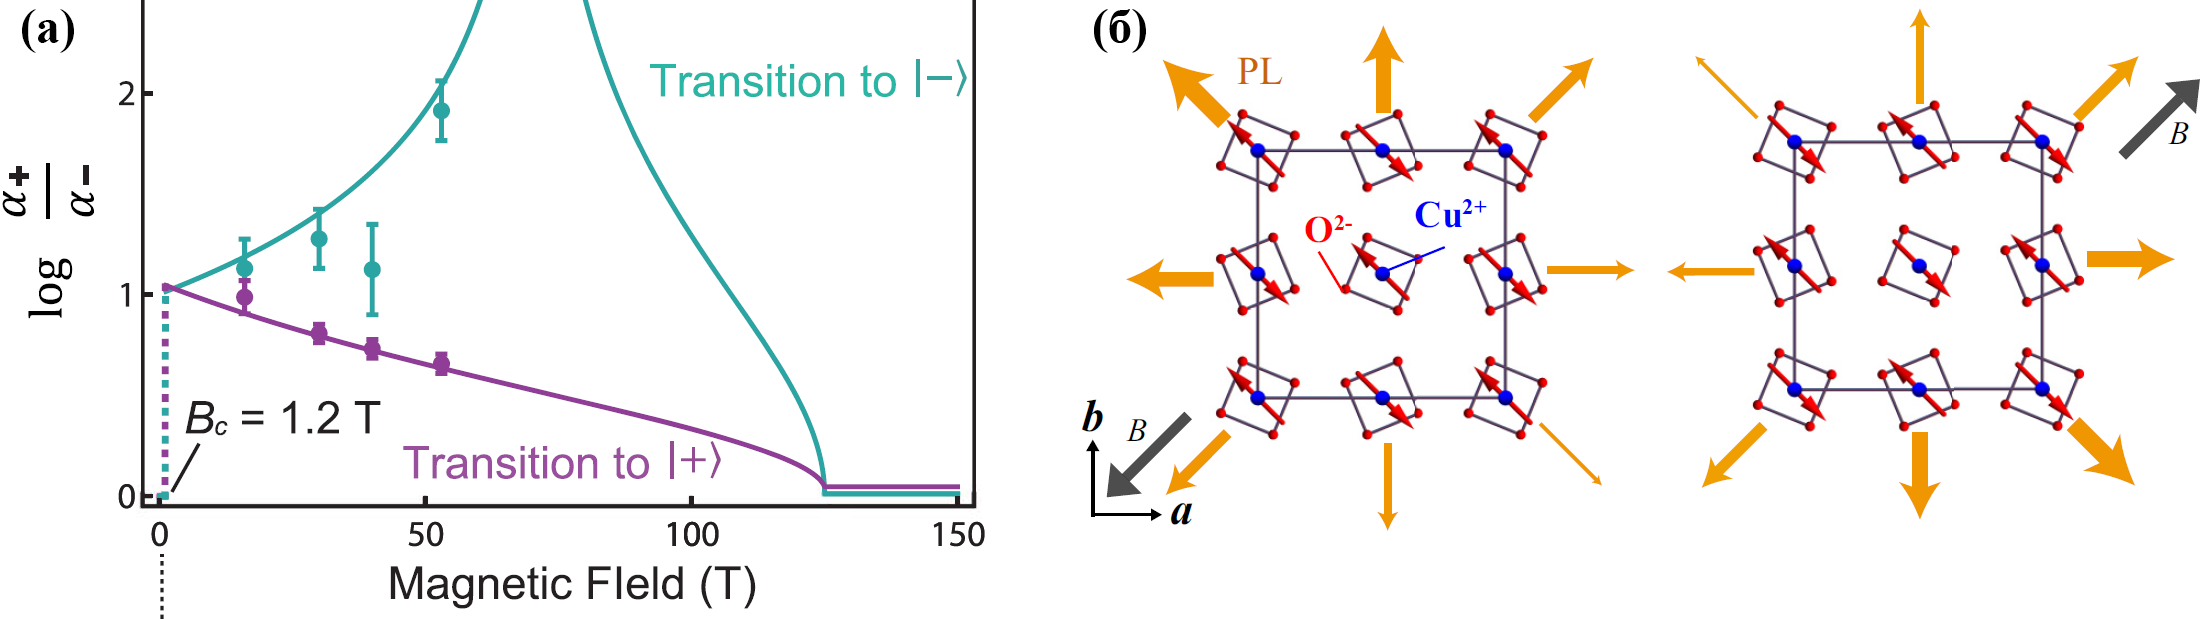
\includegraphics[scale=0.235]{ndd}
	}
\label{fig:ndd}

	\caption{(а) Расчетные (сплошная линия) и экспериментальные (точки) значения NDD на линиях бесфононного поглощения первого возбужденного дублета \cbo, расщепленного зеемановским взаимодействием при T=\SI{4.2}{\kelvin} из работы \cite{Toyoda2015}. Символами \(\alpha_+\) и \(\alpha_-\) обозначены коэффициенты поглощения света, распространяющегося в направлениях \dir{1}{$\overline{1}$}{0} и \dir{$\overline{1}$}{1}{0}. (б) Схематическая иллюстрация пространственной асимметрии люминесценции, наблюдающейся CuB2O4 (оранжевые стрелки) \cite{Toyoda2016}. Красными стрелками показаны магнитные моменты ионов \cu\ (4b) в магнитных полях.}
\end{figure}

Что касается теоретических работ по исследуемой теме, анализ экспериментальных данных проводился лишь с использованием феноменологического подхода. В статьях \cite{Bordacs2012, Kezsmarki2014, Miyahara2014} на основе анализа решений уравнений Максвелла определяется требование к компонентам магнитоэлектрического тензора, при соблюдении которого возможен эффект невзаимности: \(\chi^{me}_{\alpha\beta}+\chi^{em}_{\beta\alpha}\neq0\). Аналогичное соотношение можно получить, рассматривая перекрестные слагаемые в квадрате модуля матричного элемента перехода с одновременным действием электрического и магнитного дипольного взаимодействий: \( \left| \langle \psi_1 | \hat{H}_E + \hat{H}_M | \psi_2 \rangle \right| ^2\). В работе \cite{Nikitchenko2021} в рамках теоретико-группового подхода исследовался вопрос о том, каковы должны быть дополнительные члены в тензоре диэлектрической проницаемости для того, чтобы магнитоэлектрический эффект был возможен. Применительно к \cbo\ авторы работы \cite{Nikitchenko2021} заключили, что требуются члены, учитывающие пространственную дисперсию, т.е. зависящие от волнового вектора и индукции магнитного поля (так называемые \textbf{kB}-члены). 

Несмотря на успехи феноменологической теории магнитоэлектрических эффектов, вопрос количественной оценки компонент магнитоэлектрического тензора для определения поправок к диэлектрической проницаемости требует дополнительных исследований.

\FloatBarrier
